\subsection{Statistics of Differential Enrichment}
The \texttt{blocksStats} function is a convenient way to do statistical tests of differential enrichment between two experimental conditions, using counts in regions of interest. The windows can be relative to some genomic landmarks, like transcription start sites (TSSs), and their size can be specified with the \texttt{up} and \texttt{down} parameters. If \texttt{up} and \texttt{down} are not provided, then windows are defined by start and end coordinates. The function leverages \texttt{edgeR}'s count modelling and its adaptation of Fisher's exact test for assessing differential enrichment.  The procedure also uses Bioconductor's facilities (i.e. \texttt{countOverlaps}) for counting mapped read in regions of the genome.

\begin{Schunk}
\begin{Sinput}
 design.matrix <- matrix(c(0, -1, 0, 1), dimnames = list(names(samples.list), 
     "C-N"))
 design.matrix
\end{Sinput}
\begin{Soutput}
            C-N
PrEC input    0
PrEC IP      -1
LNCaP input   0
LNCaP IP      1
\end{Soutput}
\begin{Sinput}
 stats <- blocksStats(samples.list, gene.anno, up = 2000, down = 0, 
     seq.len = 300, design = design.matrix)
\end{Sinput}
\begin{Soutput}
Comparison of groups:  1 - -1 
\end{Soutput}
\begin{Sinput}
 stats <- stats[order(stats$`adj.p.vals_C-N`), ]
 head(stats)
\end{Sinput}
\begin{Soutput}
          chr     start       end width strand    name symbol PrEC input
8019804 chr18     99064    112217 13154      + 8019804  ROCK1        600
8015798 chr17  38802738  38821439 18702      - 8015798    ---         87
7904879  chr1 145017918 145018085   168      + 7904879    ---         21
7908529  chr1 196148257 196165896 17640      + 7908529   LHX9         16
8115391  chr5 153834725 153838017  3293      - 8115391  HAND1          8
7976848 chr14 100592279 100592359    81      + 7976848    ---         29
        PrEC IP LNCaP input LNCaP IP PrEC IP_pseudo LNCaP IP_pseudo logConc_C-N
8019804     397         686       58     399.588658      57.6237948   -16.01856
8015798      56          64      314      56.365618     311.9656941   -16.21306
7904879      13          28      153      13.085296     152.0084843   -17.78513
7908529       3          13      112       3.020114     111.2740395   -19.06788
8115391       4          28       95       4.026631      94.3841477   -18.97912
7976848      75          33        1      75.489482       0.9929602   -20.14963
        logFC_C-N  p.value_C-N adj.p.vals_C-N
8019804 -2.793764 2.911512e-64   7.268881e-60
8015798  2.468516 1.091971e-43   1.363108e-39
7904879  3.538199 3.102111e-31   2.581577e-27
7908529  5.203643 2.378716e-29   1.484676e-25
8115391  4.551106 1.238883e-23   6.185989e-20
7976848 -6.247568 2.038173e-21   8.480838e-18
\end{Soutput}
\end{Schunk}

\noindent Note that this is {\em not} a real design matrix (in a statistical sense), it is simply a way of specifying the two experiment conditions to compare (they must be 1 and -1). \\

\noindent The example above calculates statistics on regions that start 2000 bases upstream of the TSS and finish at the TSS, after the reads have been extended to being 300 bases. A coverage plot from UCSC browser illustrates the best found region.  For the output table, the read counts are scaled as if there were 10 million reads covering the regions of interest. \\

\noindent Note that this procedure only works for simple 2-group comparisons.  Using this strategy for more complicated designs requires manually creating the count tables (see \texttt{annotationCounts} below) and calling the GLM-based procedures (e.g. using real design matrices) within \texttt{edgeR}. \\


\begin{figure}[!h]
    \begin{center}
        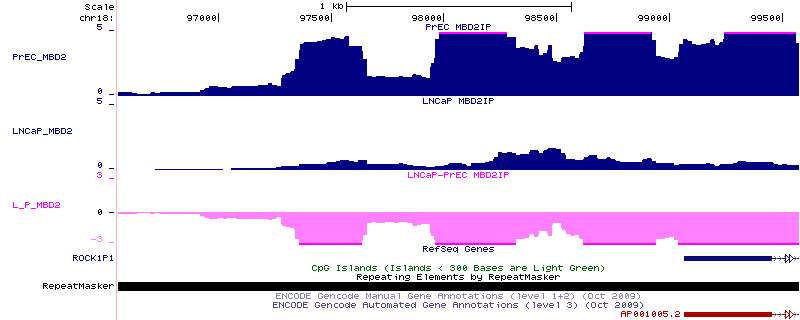
\includegraphics{rock1.png}
    \end{center}
\end{figure}

This differential enrichment strategy can be used on bins covering the entire genome.  The \texttt{genomeBlocks} function can be used to generate windows along the genome.
